%%%%%%%%%%%%%%%%%%%%%%%%%%%%%%%%%%%%%%%%%
% Beamer Presentation
% LaTeX Template
% Version 1.0 (10/11/12)
%
% This template has been downloaded from:
% http://www.LaTeXTemplates.com
%
% License:
% CC BY-NC-SA 3.0 (http://creativecommons.org/licenses/by-nc-sa/3.0/)
%
%%%%%%%%%%%%%%%%%%%%%%%%%%%%%%%%%%%%%%%%%

%----------------------------------------------------------------------------------------
%	PACKAGES AND THEMES
%----------------------------------------------------------------------------------------

\documentclass{beamer}

\mode<presentation> {

% The Beamer class comes with a number of default slide themes
% which change the colors and layouts of slides. Below this is a list
% of all the themes, uncomment each in turn to see what they look like.

\usetheme{default}
% \usetheme{AnnArbor}
% \usetheme{Antibes}
% \usetheme{Bergen}
% \usetheme{Berkeley}
%\usetheme{Berlin}
%\usetheme{Boadilla}
%\usetheme{CambridgeUS}
% \usetheme{Copenhagen}
% \usetheme{Darmstadt}
% \usetheme{Dresden}
% \usetheme{Frankfurt}
%\usetheme{Goettingen}
%\usetheme{Hannover}
%\usetheme{Ilmenau}
%\usetheme{JuanLesPins}
%\usetheme{Luebeck}
% \usetheme{Madrid}
%\usetheme{Malmoe}
%\usetheme{Marburg}
%\usetheme{Montpellier}
%\usetheme{PaloAlto}
%\usetheme{Pittsburgh}
%\usetheme{Rochester}
%\usetheme{Singapore}
%\usetheme{Szeged}
%\usetheme{Warsaw}

% As well as themes, the Beamer class has a number of color themes
% for any slide theme. Uncomment each of these in turn to see how it
% changes the colors of your current slide theme.

%\usecolortheme{albatross}
%\usecolortheme{beaver}
%\usecolortheme{beetle}
%\usecolortheme{crane}
%\usecolortheme{dolphin}
%\usecolortheme{dove}
%\usecolortheme{fly}
%\usecolortheme{lily}
%\usecolortheme{orchid}
%\usecolortheme{rose}
%\usecolortheme{seagull}
%\usecolortheme{seahorse}
%\usecolortheme{whale}
%\usecolortheme{wolverine}

%\setbeamertemplate{footline} % To remove the footer line in all slides uncomment this line
\setbeamertemplate{footline}[page number] % To replace the footer line in all slides with a simple slide count uncomment this line

\setbeamertemplate{navigation symbols}{} % To remove the navigation symbols from the bottom of all slides uncomment this line
}

\usepackage{graphicx} % Allows including images
\usepackage{booktabs} % Allows the use of \toprule, \midrule and \bottomrule in tables
%\usepackage {tikz}
\usepackage{subcaption}
\usepackage{tkz-graph}
\usepackage{tabularx}
\usepackage{threeparttable}  

\GraphInit[vstyle = Shade]
\tikzset{
  LabelStyle/.style = { rectangle, rounded corners, draw,
                        minimum width = 2em, fill = yellow!50,
                        text = red, font = \bfseries },
  VertexStyle/.append style = { inner sep=5pt,
                                font = \normalsize\bfseries},
  EdgeStyle/.append style = {->, bend left} }
\usetikzlibrary {positioning}
%\usepackage {xcolor}
\definecolor {processblue}{cmyk}{0.96,0,0,0}
%----------------------------------------------------------------------------------------
%	TITLE PAGE
%----------------------------------------------------------------------------------------

\title[Short title]{OOV Handling by Learning Subword using CNN based N-grams} % The short title appears at the bottom of every slide, the full title is only on the title page

\author{Yonathan Purbo Santosa} % Your name
\institute[Institut f{\"u}r Informatik] % Your institution as it will appear on the bottom of every slide, may be shorthand to save space
{
Institut f{\"u}r Informatik\\
Rheinische Friedrich-Wilhelms-Universit{\"a}t Bonn % Your institution for the title page
\medskip
}
\date{November 13, 2019} % Date, can be changed to a custom date

\begin{document}

\begin{frame}
\titlepage % Print the title page as the first slide
\end{frame}

\begin{frame}
\frametitle{Overview} % Table of contents slide, comment this block out to remove it
\tableofcontents % Throughout your presentation, if you choose to use \section{} and \subsection{} commands, these will automatically be printed on this slide as an overview of your presentation
\end{frame}

%----------------------------------------------------------------------------------------
%	PRESENTATION SLIDES
%----------------------------------------------------------------------------------------

%----------------------------------------------------------------------------------------
%	INTRODUCTION
%----------------------------------------------------------------------------------------
\section{Introduction}
\begin{frame}{Introduction}
    \textbf{Why OOV handling is needed?}\\~\\

    \begin{itemize}
        \item Word embedding prefers large corpus \cite{size2018kutuzov}
        \item Language itself is creative and changing overtime
        \cite{forrester2008abrief, speech2009Jurafsky};
        \item Some word embedding has no OOV handling method
        \cite{polyglot2013alrfo, dict2vect2017tissier, efficient2013mikolov}; and 
        \item Improvements should be able to be achieved over using
        random or unknown embedding for OOV.
    \end{itemize}
\end{frame}

%------------------------------------------------
\begin{frame}{Introduction}
    \textbf{Previous state-of-the-art \textsc{Mimick}}\\~\\

    \begin{figure}[H]
        \centering
        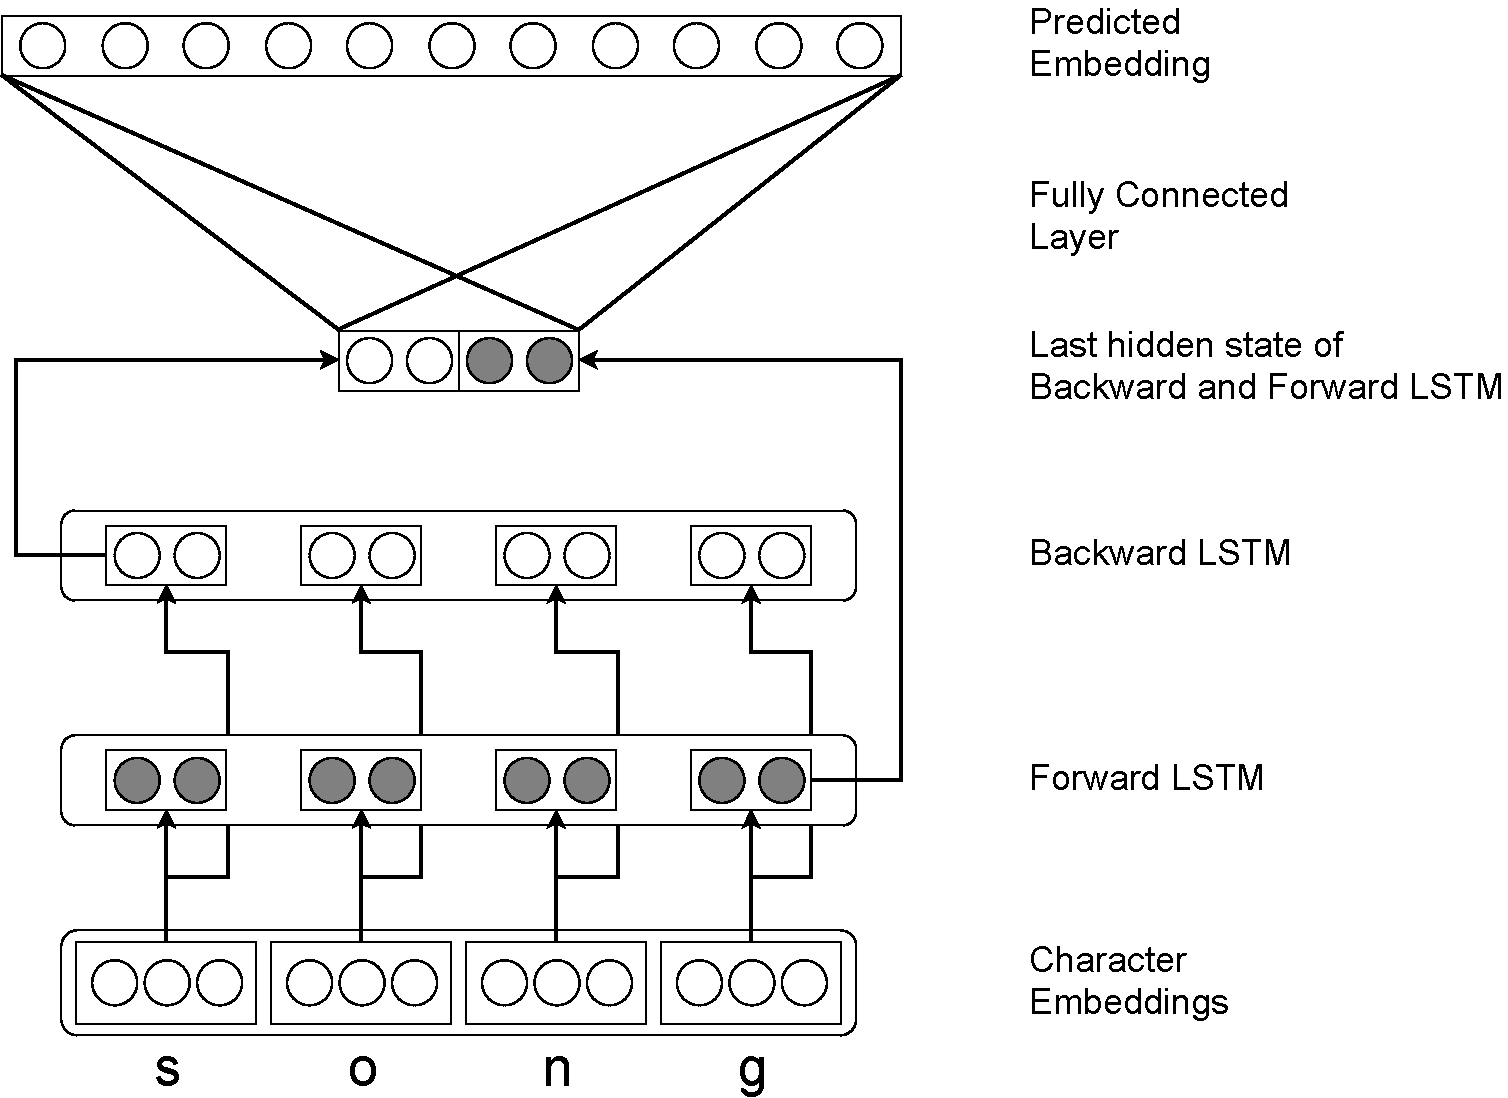
\includegraphics[width=70mm]{images/mimick}
        \caption{\textsc{Mimick} Architecture}
    \end{figure}
\end{frame}

%------------------------------------------------

\begin{frame}{Introduction}
    \textbf{What could be the problem with \textsc{Mimick}?}\\~\\

    \begin{itemize}
        \item \textsc{Mimick} used the last hidden state of bi-LSTM to
        infer OOV embedding \cite{mimicking2017Pinter};
        \item By default, LSTM has a cell gate that could split
        the graph of the hidden unit when the input or previous state
        triggers it
        \item The last hidden state only encoded the recent sequence
        \item There is evidence that CNN can performs better than RNN
        and LSTM in sequence modeling \cite{empirical2018shaujie}
    \end{itemize}
\end{frame}




%------------------------------------------------

%----------------------------------------------------------------------------------------
%	OBJECTIVE
%----------------------------------------------------------------------------------------
\section{Objective}
\begin{frame}{Objective}
    \begin{itemize}
        \item Similar with \textsc{Mimick}, this problem is tackled
        from quasi-generative perspective
        \item Instead of using bi-LSTM, CNN that based on n-grams can
        be used to learn character sequence
        \cite{convolutional2014kim}.
        \item CNN N-grams can process different length sequence using
        max-over-time pooling.
        \item For each kernel $K$, an input that has similar features
        to the kernel can still gives a high response.
    \end{itemize}
\end{frame}

%------------------------------------------------
%----------------------------------------------------------------------------------------
%	CNN N-grams for OOV handling
%----------------------------------------------------------------------------------------
\section{CNN N-grams for OOV handling}
\begin{frame}{CNN N-grams for OOV handling}
    \begin{itemize}
        \item Given a word and its embedding $(w_i, e_i)$
        \item The word is transformed into sequence of character
        embedding $g_i \in \mathcal{G}$
        \begin{align*}
            h &: w_i \rightarrow [c_1, c_2,\dots, c_n] \rightarrow [g_1, g_2,\dots,g_n]
        \end{align*}
        \item The sequence of character embedding then processed by
        the OOV handling model to predict the embedding $\tilde{e}_i$
        \begin{align*}
            OOV_{model}(w_i) = \tilde{e}_i
        \end{align*}
    \end{itemize}
\end{frame}

%------------------------------------------------


\begin{frame}{CNN N-grams for OOV handling}
    \begin{figure}[H]
        \centering
        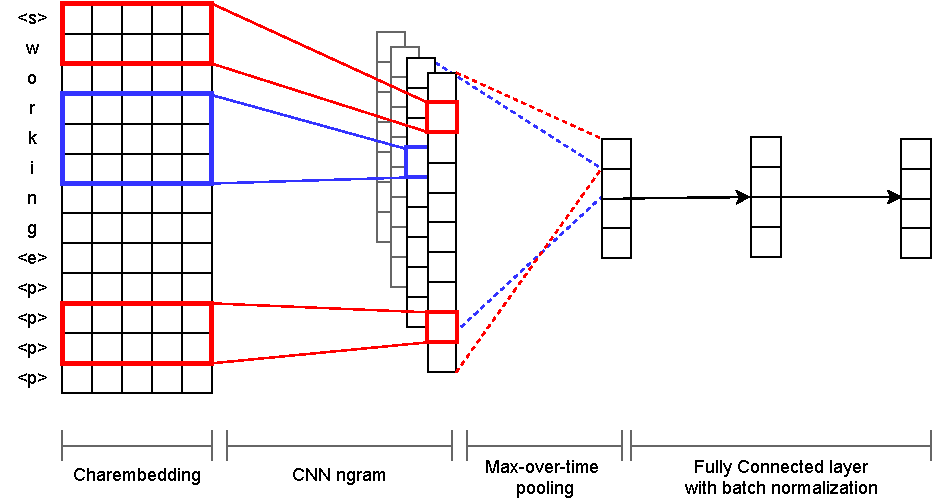
\includegraphics[width=70mm]{images/model_batchnorm}
        \caption{CNN N-grams for OOV Handling Architecture}
    \end{figure}
    \begin{itemize}
        \item $[2, 3, 4, 5, 6, 7]$-grams were used as the feature extractor
        \item ReLU activation function was used before the
        max-over-time pooling
    \end{itemize}
\end{frame}

%------------------------------------------------

\begin{frame}{CNN N-grams for OOV handling}
    \begin{itemize}
        \item \textit{Hardtanh} is used for predicting embedding
        \item The predicted embedding was used for calculating the
        deviation from the original embedding $e_i$ by using MSE
        \begin{align*}
            \mathcal{L} = \frac{1}{2}\Vert e_i - \tilde{e}_i \Vert^2_2
        \end{align*}
    \end{itemize}
    Both model trained with three word embedding:
    \begin{itemize}
        \item Polyglot ($\sim$100k words)
        \item Word2vec first 40k with reduction ($\sim$35k words). If the word
        contain underscore ``\_'' or ``http'' then it will be
        removed
        \item Dict2vec 100 dimension ($\sim$50k words)
    \end{itemize}
\end{frame}
%------------------------------------------------

\begin{frame}{CNN N-grams for OOV handling}

    \begin{table}[]
        \centering
        \caption{OOV Handling Model Parameters}
        \label{tab:hyperparameter}
        \begin{tabular}{@{}lcc@{}}
            \toprule
            \textbf{Hyperparameter} & \multicolumn{1}{c}{\textbf{\textsc{Mimick}}} & \multicolumn{1}{c}{\textbf{CNN}} \\ \midrule
            Train-Val split & \multicolumn{2}{c}{$80\%$; $20\%$}\\
            Batch size & \multicolumn{2}{c}{64} \\
            Epoch & \multicolumn{2}{c}{100} \\
            Momentum & \multicolumn{2}{c}{0.5} \\
            Learning Rate ($\eta$) & [0.01; 0.1] & 0.1 \\
            Dropout & 0 & 0.5 \\
            Num features & [50; 100; 200; 300] & [20; 50; 100; 150] \\ \bottomrule
        \end{tabular}
    \end{table}
\end{frame}
%----------------------------------------------------------------------------------------
%	Evaluation on Downstream Tasks
%----------------------------------------------------------------------------------------
\section{Evaluation on Downstream Tasks}
\begin{frame}{Evaluation on Downstream Tasks}
    \textbf{Part-of-Speech Tagging}
    \begin{itemize}
        \item Using brown POStagging datasets from NLTK\footnote{Available at \url{https://www.nltk.org/}}
        \item Following POS-tagger model from Ling et al. (2015) \cite{finding2015ling}
        \item Sentence length limited to 5 words
        \item There are 3 different setup for POS-tagger: Freeze,
        Continuous, Continuous with Trainable Embedding
        \item LogSoftmax is used for classifying the tags
    \end{itemize}
\end{frame}
%------------------------------------------------

\begin{frame}{Evaluation on Downstream Tasks}
    \textbf{Part-of-Speech Tagging}
    \begin{figure}[H]
        \centering
        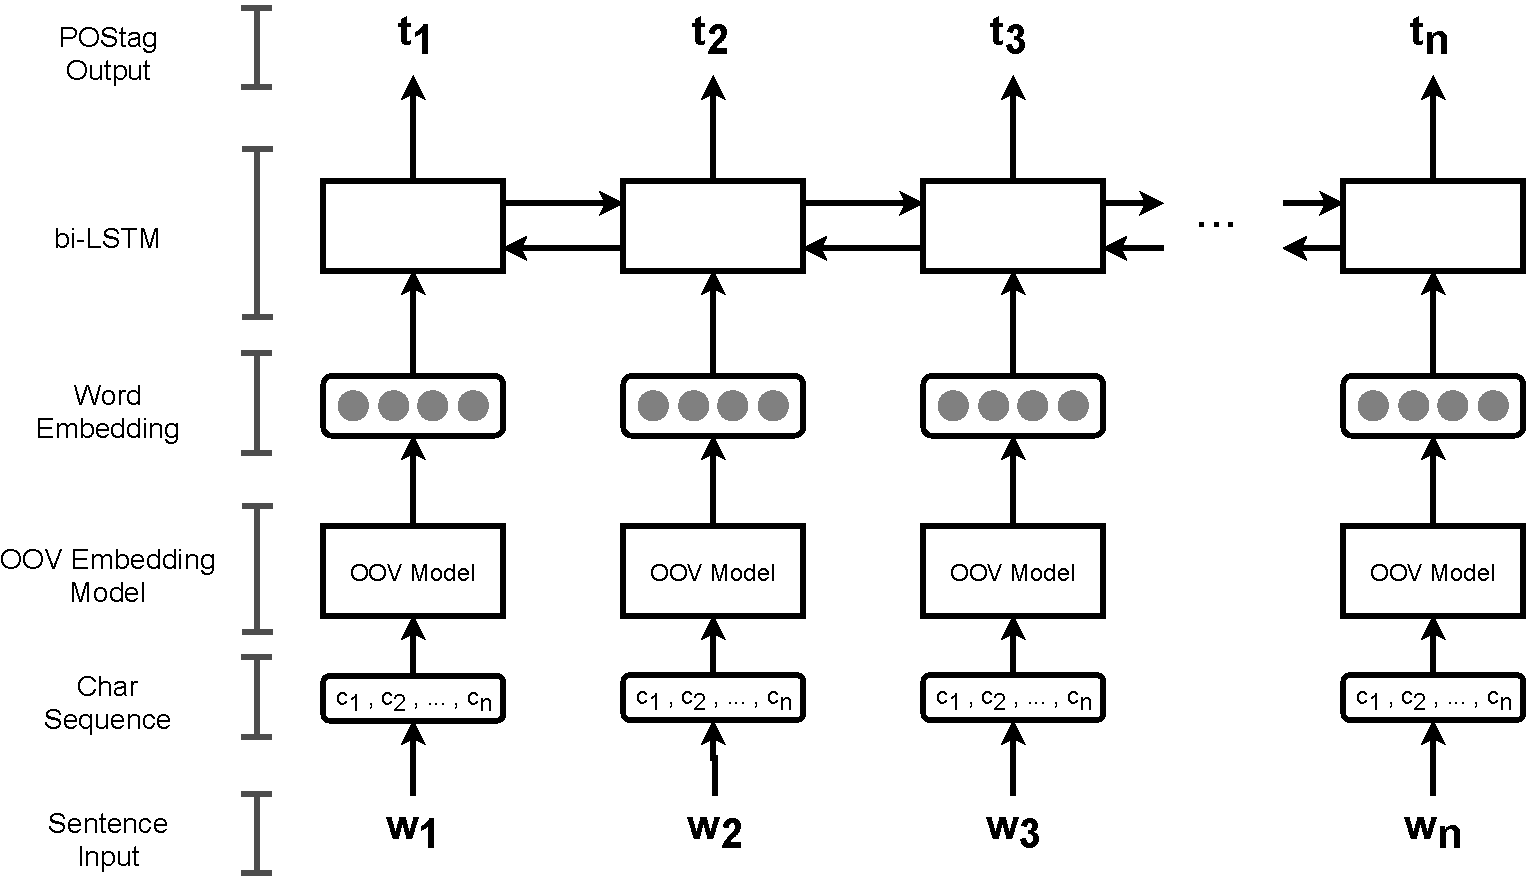
\includegraphics[width=90mm]{images/postag}
        \caption{POS-tagger Model}
    \end{figure}
\end{frame}
%------------------------------------------------
\begin{frame}{Evaluation on Downstream Tasks}
    \textbf{Part-of-Speech Tagging Result Random}
    \begin{figure}[H]
        \centering
        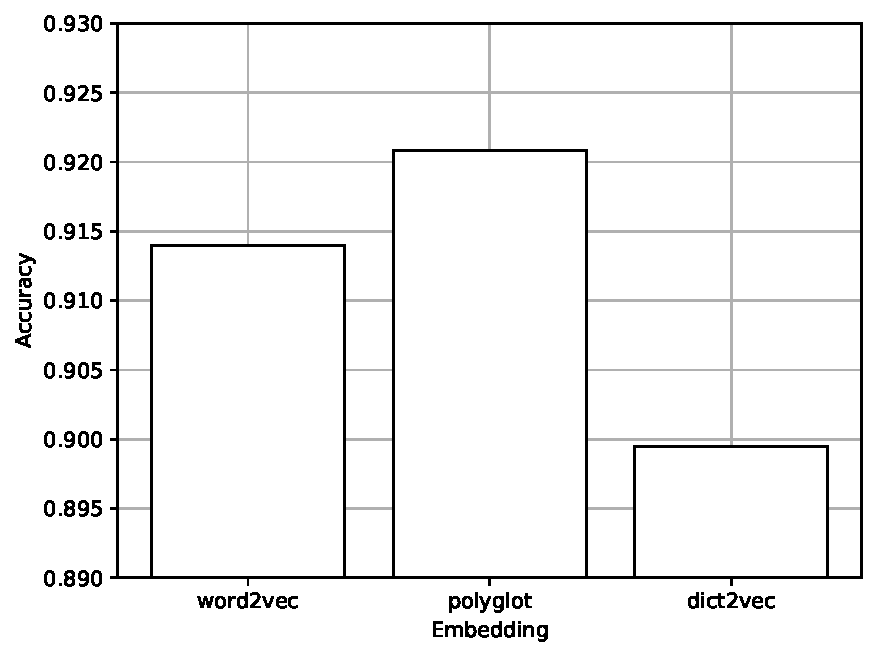
\includegraphics[width=70mm]{images/random_graph}
        \caption{Random OOV Embedding}
    \end{figure}
\end{frame}
%------------------------------------------------
\begin{frame}{Evaluation on Downstream Tasks}
    \textbf{Part-of-Speech Tagging Result Freeze}
    \begin{figure}[H]
        \centering
        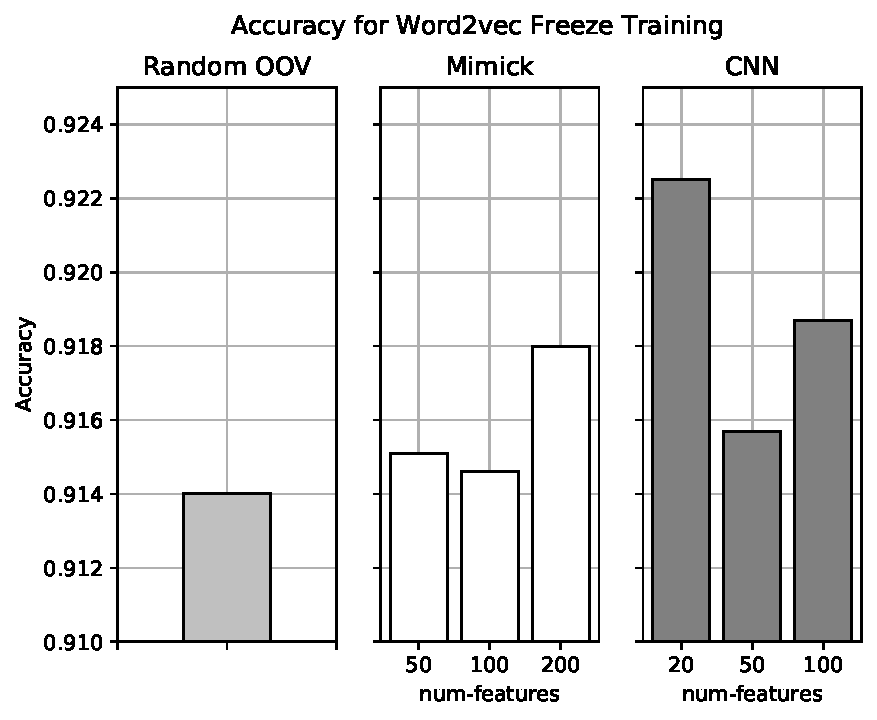
\includegraphics[width=70mm]{images/freeze_word2vec}
    \end{figure}
\end{frame}
%------------------------------------------------
\begin{frame}{Evaluation on Downstream Tasks}
    \textbf{Part-of-Speech Tagging Result Freeze}
    \begin{figure}[H]
        \centering
        \begin{minipage}{.48\textwidth}
            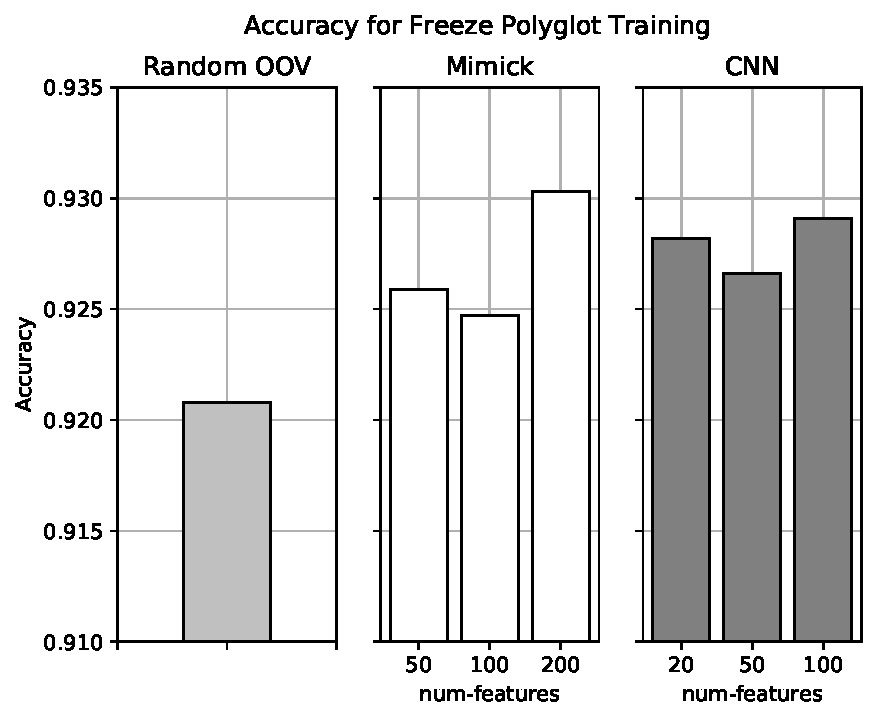
\includegraphics[width=\linewidth]{images/freeze_polyglot}
        \end{minipage}
        \begin{minipage}{.48\textwidth}
            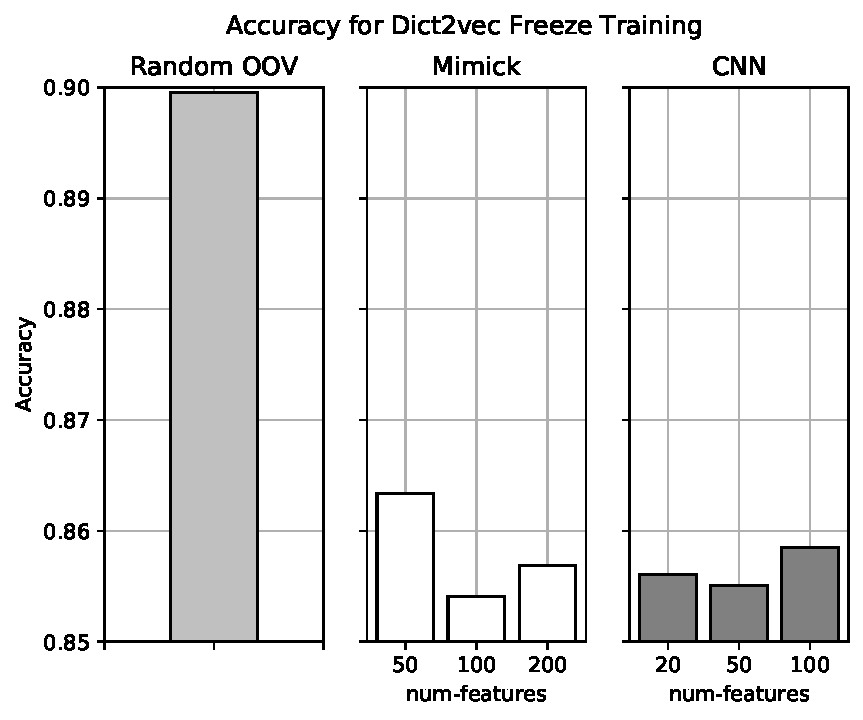
\includegraphics[width=\linewidth]{images/freeze_dict2vec}
        \end{minipage}
    \end{figure}
\end{frame}
%------------------------------------------------

\begin{frame}{Evaluation on Downstream Tasks}
    \textbf{Part-of-Speech Tagging Result Continuous}
    \begin{figure}[H]
        \centering
        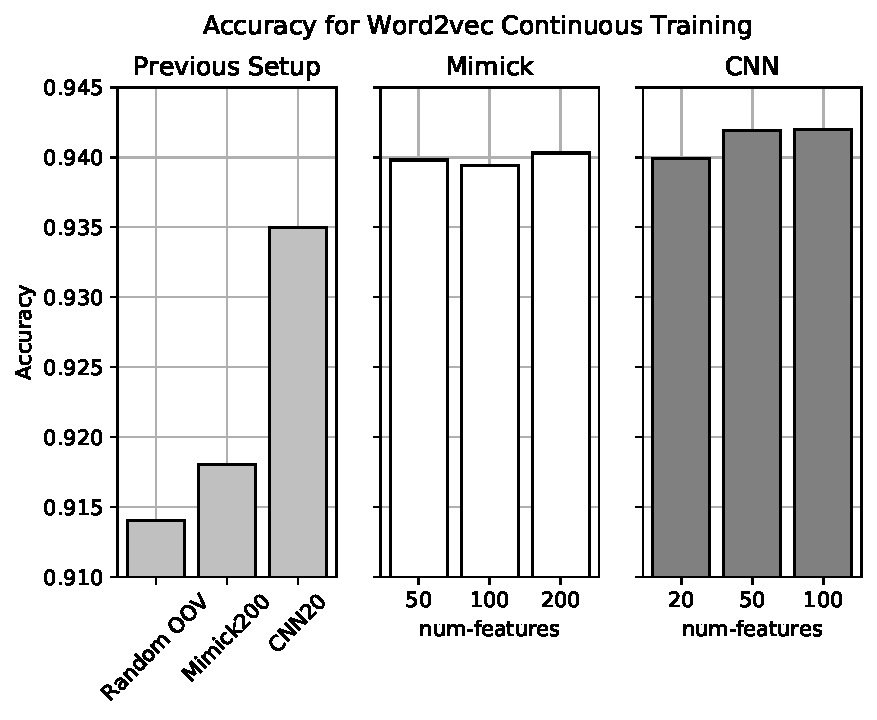
\includegraphics[width=70mm]{images/continuous_word2vec}
    \end{figure}
\end{frame}
%------------------------------------------------
\begin{frame}{Evaluation on Downstream Tasks}
    \textbf{Part-of-Speech Tagging Result Continuous}
    \begin{figure}[H]
        \centering
        \begin{minipage}{.48\textwidth}
            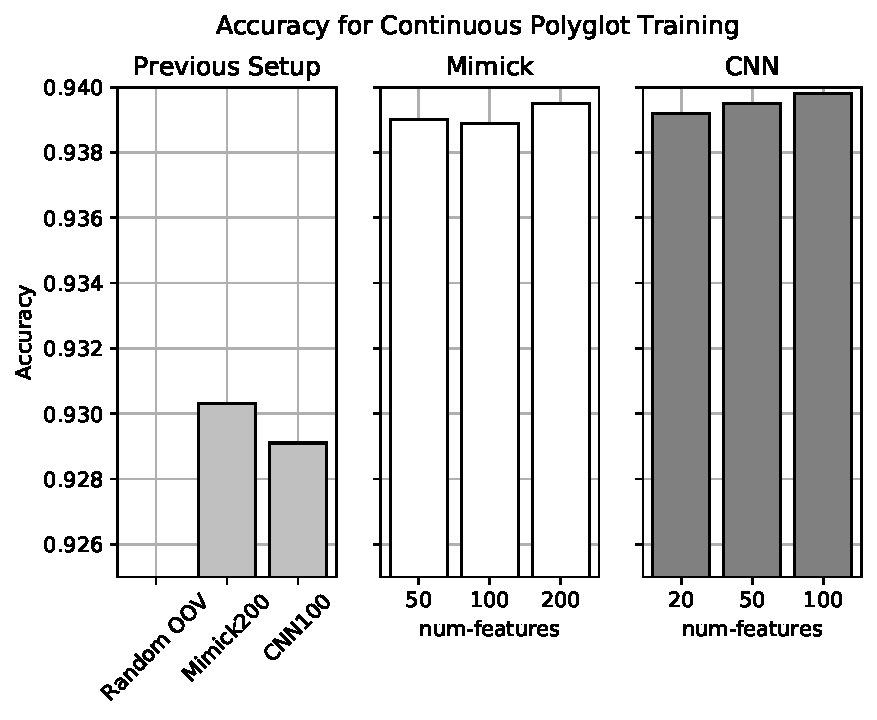
\includegraphics[width=\linewidth]{images/continuous_polyglot}
        \end{minipage}
        \begin{minipage}{.48\textwidth}
            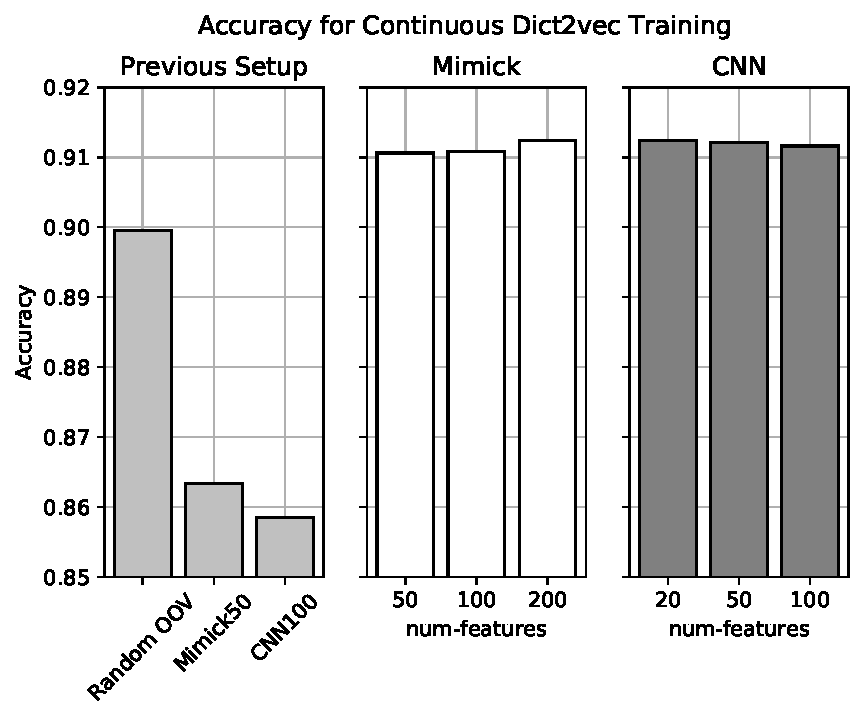
\includegraphics[width=\linewidth]{images/continuous_dict2vec}
        \end{minipage}
    \end{figure}
\end{frame}
%------------------------------------------------
\begin{frame}{Evaluation on Downstream Tasks}
    \textbf{Part-of-Speech Tagging Result Continuous with Trainable Embedding}
    \begin{figure}[H]
        \centering
        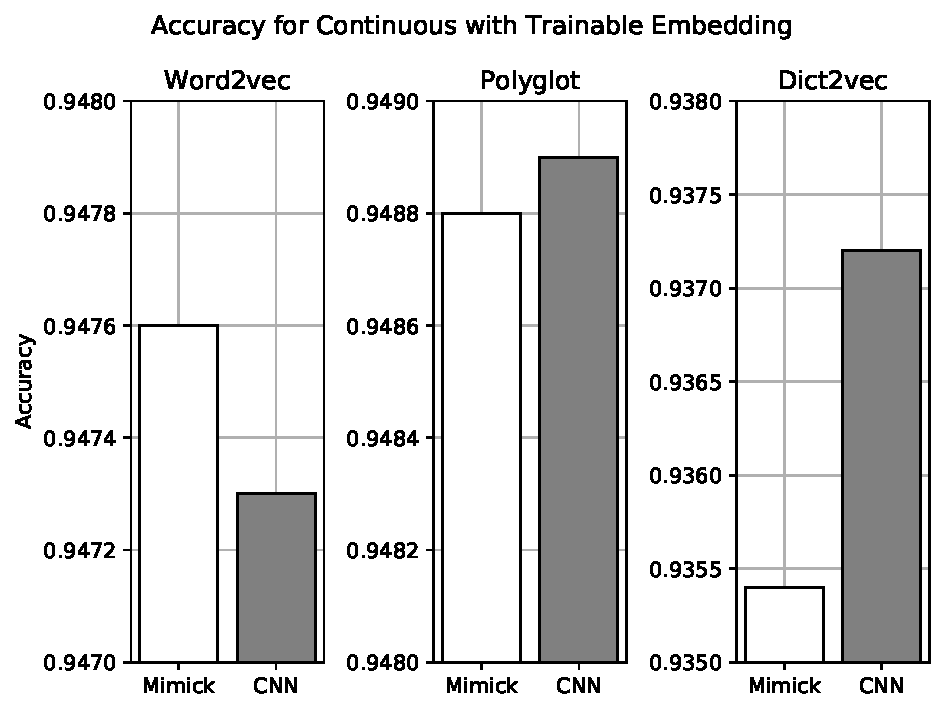
\includegraphics[width=70mm]{images/train_embed}
    \end{figure}
\end{frame}
%------------------------------------------------
\begin{frame}{Evaluation on Downstream Tasks}
    \textbf{Word Similarity}
    \begin{itemize}
        \item Using 12 different datasets to increase the data test size
        \item Only OOV embedding was inferred from the OOV handling model
        \item The cosine distance of a given pairs was calculated and
        compared with the dataset with Spearman's rank correlation
        coefficient.
    \end{itemize}
\end{frame}

%------------------------------------------------
\begin{frame}{Evaluation on Downstream Tasks}
    \textbf{Word Similarity Results}
    \begin{table}[!ht]
        \footnotesize
        \begin{center}
        \begin{threeparttable} 
          \caption{Word Similarity Task Results (word2vec)}
          ~\\
          \label{tab:wordsim:word2vec}
          \begin{tabular}{l|c|c|c|c|c}
            \textbf{Dataset} & \textbf{OOV} & \textbf{Invocab} & \textbf{OOV Ratio} & \textbf{Mimick}\tnote{*} & \textbf{CNN}\tnote{*}\\
            \hline
            card & 989 & 317 & 75.73\% & \textbf{52.27} & 27.25\\
            mc30 & 4 & 35 & 10.26\% & 748.11 & \textbf{758.79}\\
            men & 83 & 668 & 11.05\% & \textbf{672.54} & 664.64\\
            mturk287 & 97 & 402 & 19.44\% & 518.15 & \textbf{519.76}\\
            mturk771 & 18 & 1095 & 1.62\% & \textbf{657.93} & 657.04\\
            rg65 & 2 & 46 & 4.17\% & 709.77 & \textbf{732.61}\\
            rwstanford & 1494 & 1457 & 50.63\% & \textbf{233.83} & 217.47\\
            simlex & 20 & 1008 & 1.95\% & 422.77 & \textbf{425.90}\\
            simverb & 90 & 737 & 10.88\% & \textbf{302.37} & 292.91\\
            verb143 & 4 & 113 & 3.42\% & 467.60 & \textbf{478.25}\\
            wordsim & 15 & 422 & 3.43\% & \textbf{658.92} & 648.25\\
            yp130 & 6 & 141 & 4.08\% & \textbf{460.32} & 443.22\\
            \hline
            \multicolumn{4}{r|}{\textbf{average}} & \textbf{492.05} & 488.84\\
          \end{tabular}
          \begin{tablenotes}
            \item[*] multiplied by 1000
          \end{tablenotes}
        
        \end{threeparttable} 
        \end{center}
        \end{table}
\end{frame}

%------------------------------------------------
\begin{frame}{Evaluation on Downstream Tasks}
    \textbf{Word Similarity Results}
    \begin{table}[!ht]
        \footnotesize
        \begin{threeparttable} 
        \begin{center}
          \caption{Word Similarity Task Results (polyglot)}
          ~\\
          \label{tab:wordsim:polyglot}
          \begin{tabular}{l|c|c|c|c|c}
            \textbf{Dataset} & \textbf{OOV} & \textbf{Invocab} & \textbf{OOV Ratio} & \textbf{Mimick}\tnote{*} & \textbf{CNN}\tnote{*}\\
            \hline
            card & 864 & 442 & 66.16\% & \textbf{128.93} & 114.11\\
            mc30 & 1 & 38 & 2.56\% & 605.25 & 605.25\\
            men & 14 & 737 & 1.86\% & 490.57 & \textbf{492.17}\\
            mturk287 & 76 & 423 & 15.23\% & 443.31 & \textbf{458.81}\\
            mturk771 & 3 & 1110 & 0.27\% & \textbf{432.48} & 432.20\\
            rg65 & 1 & 47 & 2.08\% & 531.59 & \textbf{524.77}\\
            rwstanford & 999 & 1952 & 33.85\% & 272.33 & \textbf{290.78}\\
            simlex & 4 & 1024 & 0.39\% & 232.20 & \textbf{234.16}\\
            simverb & 53 & 774 & 6.41\% & \textbf{137.01} & 134.42\\
            verb143 & 0 & 117 & 0.00\% & 335.81 & 335.81\\
            wordsim & 0 & 437 & 0.00\% & 412.83 & 412.83\\
            yp130 & 5 & 142 & 3.40\% & \textbf{44.76} & 44.62\\
            \hline
            \multicolumn{4}{r|}{average} & 338.92 & \textbf{339.99}\\
          \end{tabular}
          \begin{tablenotes}
            \item[*] multiplied by 1000
          \end{tablenotes}
        \end{center}
      \end{threeparttable} 
      \end{table}
\end{frame}

%------------------------------------------------
\begin{frame}{Evaluation on Downstream Tasks}
    \textbf{Word Similarity Results}
    \begin{table}[!ht]
        \footnotesize
        \begin{threeparttable} 
        \begin{center}
          \caption{Word Similarity Task Results (Dict2vec)}
          ~\\
          \label{tab:wordsim:dict2vec}
          \begin{tabular}{l|c|c|c|c|c|c}
            \textbf{Dataset} & \textbf{OOV} & \textbf{Invocab} &
            \textbf{OOV Ratio} & \textbf{Random}\tnote{*} &
            \textbf{Mimick}\tnote{*} & \textbf{CNN}\tnote{*}\\
            \hline
            card & 828 & 478 & 63.40\% & 48.07 & 80.89 & \textbf{95.32}\\
            mc30 & 0 & 39 & 0.00\% & 847.57 & 847.57 & 847.57\\
            men & 1 & 750 & 0.13\% & 713.16 & 723.63 & \textbf{723.89}\\
            mturk287 & 2 & 497 & 0.40\% & 652.27 & \textbf{655.32} & 653.13\\
            mturk771 & 0 & 1113 & 0.00\% & 683.91 & 683.91 & 683.91\\
            rg65 & 0 & 48 & 0.00\% & 832.86 & 832.86 & 832.86\\
            rwstanford & 619 & 2332 & 20.98\% & 214.60 & \textbf{403.79} & 400.27\\
            simlex & 3 & 1025 & 0.29\% & 454.80 & \textbf{460.66} & 459.87\\
            simverb & 24 & 803 & 2.90\% & 375.15 & 390.09 & \textbf{393.39}\\
            verb143 & 0 & 117 & 0.00\% & 187.82 & 187.82 & 187.82\\
            wordsim & 18 & 419 & 4.12\% & 642.71 & 718.72 & \textbf{723.72}\\
            yp130 & 2 & 145 & 1.36\% & 577.76 & 621.38 & \textbf{621.75}\\
            \hline
            \multicolumn{4}{r|}{average} & 519.22 & 550.55 & \textbf{551.96}\\
          \end{tabular}
          \begin{tablenotes}
            \item[*] multiplied by 1000
          \end{tablenotes}
        \end{center}
      \end{threeparttable} 
      \end{table}
\end{frame}
%----------------------------------------------------------------------------------------
%	Conclusion
%----------------------------------------------------------------------------------------
\section{Conclusion and Future Works}
\begin{frame}{Conclusion}
    % \textbf{OOV Handling Model}
    \begin{itemize}
        \item Machine learning can be
        used to generate OOV embedding
        \item Compared to random OOV embedding, machine learning
        method has higher performance in downstream tasks
        \item CNN generally performs better than bi-LSTM for POS-tagging and word
        similarity tasks
        \begin{itemize}
            \item \textsc{Mimick} has higher accuracy in
            POS-tagging:\\
            when the pre-trained embedding \& the OOV handling model
            are non-trainable (\textit{out-of-the-box})
            \item CNN N-grams has higher accuracy in POS-tagging:\\
            when both pre-trained embedding and the OOV handling model
            are trainable
            \item Despite that \textsc{Mimick} preforms better
            \textit{out-of-the-box} for POS-tagging, this was not the case for word
            similarity task
        \end{itemize}
    \end{itemize}
\end{frame}

\begin{frame}{Future Works}
    % \textbf{OOV Handling Model}
    \begin{itemize}
        \item A function that can generate an entire embedding
        \item Save space (e.g. word2vec 3 million words and phrases is
        around 2GB)
        \item Save computational needs for new entries cases
    \end{itemize}
\end{frame}

\begin{frame}
    \Huge{\centerline{Thank you for your attention!}}
\end{frame}
    
\begin{frame}
    \frametitle{References}
    \fontsize{8}{4}\selectfont
    \begin{thebibliography}{99} % Beamer does not support BibTeX so references must be inserted manually as below
        \bibitem[1]{size2018kutuzov} A. Kutuzov and M. Kunilovskaya (2018)
        \newblock Size vs. structure in training corpora
        for word embedding models: Araneum russicum maximum and russian national
        corpus
        \newblock \emph{Analysis of Images, Social Networks and Texts 2018}
        \newblock Springer International Publishing
        
        \bibitem[2]{forrester2008abrief} Julie C. Forrester (2008)
        \newblock A Brief Overview of English as a Language in Change
        \newblock \emph{Canadian Center of Science and Education 2008}, Vol. 4(4) 
    
        \bibitem[3]{speech2009Jurafsky} Daniel Jurafsky and James H. Martin (2009)
        \newblock Speech and Language Processing (3rd Edition)
        \newblock \emph{Prentice-Hall, Inc.}
    
        \bibitem[4]{polyglot2013alrfo} Rami Al-Rfou, Bryan Perozzi,
        and Steven Skiena (2010)
        \newblock Polyglot: Distributed Word Representations for Multilingual {NLP}
        \newblock \emph{Proceedings of the Seventeenth Conference on Computational Natural Language Learning}
        \newblock Association for Computational Linguistics
    
        \bibitem[5]{dict2vect2017tissier} Julien Tissier, Christophe Gravier, and Amaury Habrard (2017)
        \newblock Dict2vec : Learning Word Embeddings using Lexical Dictionaries 
        \newblock \emph{Proceedings of the 2017 Conference on Empirical Methods in Natural Language Processing}, 254--263
        \newblock Association for Computational Linguistics    
    \end{thebibliography}
\end{frame}

% ------------------------------------------------
    

% %------------------------------------------------
% \begin{frame}
%     \frametitle{References}
%     \fontsize{8}{4}\selectfont
%     \begin{thebibliography}{99} % Beamer does not support BibTeX so references must be inserted manually as below
%         \bibitem[Sharma et al., 2015]{sharma} Raksha Sharma, Mobit Gupta, Astha Agarwal, and Pushpak Bhattacharyya (2015)
%         \newblock Adjective Intensity and Sentiment Analysis
%         \newblock \emph{Proceedings of the 2015 Conference on Empirical Methods in Natural Language Processing}, 2520--2526   

%         \bibitem[Mikolov et al., 2013]{mikolov} Tomas Mikolov, Kai Chen, Greg Corrado, and Jeffrey Dean (2013)
%         \newblock Efficient Estimation of Word Representations in Vector Space
%         \newblock \emph{http://arxiv.org/abs/1301.3781}
    
%         \bibitem[Zhu et al., 2014]{zhu} Xiaodan Zhu, Svetlana Kiritchenko, and Saif Mohammad (2014)
%         \newblock Recent improvements in the sentiment analysis of tweets.
%         \newblock \emph{Proceedigns of SemEval-2014}, 443--447
        
%     \end{thebibliography}
\begin{frame}
    \frametitle{References}
    \fontsize{8}{4}\selectfont
    \begin{thebibliography}{99} % Beamer does not support BibTeX so references must be inserted manually as below
        \bibitem[6]{mimicking2017Pinter} Yuval Pinter, Robert Guthrie,
         and Jacob Eisenstein (2017)
        \newblock Mimicking Word Embeddings using Subword RNNs
        \newblock \emph{Proceedings of the 2017 Conference on Empirical Methods in Natural Language Processing} 

        \bibitem[7]{convolutional2014kim} Yoon Kim (2014)
        \newblock Convolutional Neural Networks for Sentence Classification
        \newblock \emph{Proceedings of the 2014 Conference on Empirical Methods in Natural Language Processing}, 1746--1751
    
        \bibitem[8]{finding2015ling} Wang Ling, Chris Dyer, Alan W.
        Black, Isabel Trancoso, Ramon Fermandez, Silvio Amir, Luis
        Marujo, and Tiago Luis (2015)
        \newblock Finding Function in Form: Compositional Character Models for Open Vocabulary Word Representation
        \newblock \emph{Proceedings of the 2015 Conference on Empirical Methods in Natural Language Processing} 1520--1530
    \end{thebibliography}
    
\end{frame}



\end{document}

